\section{IR-analyse af stofferne paracetamol, ibuprofen og R-limonen}
Vi vil i dette afsnit se nærmere på hvordan man i praksis bestemmer hvilket stof et bestemt IR-spektrogram hører til. Der vil ses på de tre stoffer: paracetamol, som er et udbredt smertestillende middel, ibuprofen, der også er smertestillende og til sidst stoffet R-limonen, som er en farveløs væske der ved stuetemperatur dufter kraftigt af appelsin (FODNOTE WIKI). Vi har tre forskellige stoffer vi skal tildele til tre forskellige IR-spektre. Man kan indledningsvist se på molekylernes opbygning og gøre det klart for sig selv, hvilke steder man forventer at se absorption. 
\\

Der kigges da på de funktionelle grupper som de tre stoffer indeholder

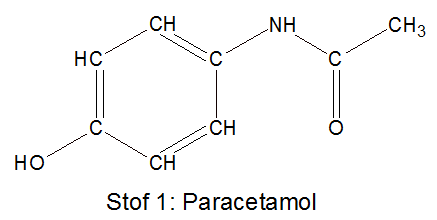
\includegraphics[scale=0.5]{Billeder/paracetamol}
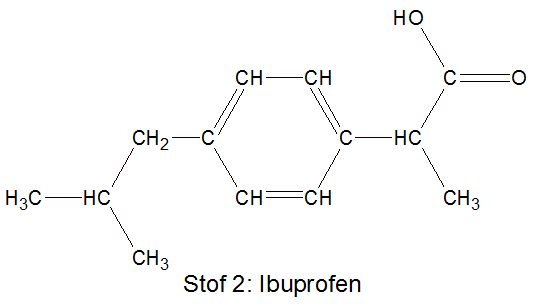
\includegraphics[scale=0.5]{Billeder/ibuprofen}
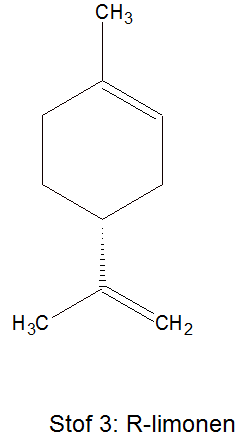
\includegraphics[scale=0.5]{Billeder/Rlimonen}
\begin{enumerate}
\item[\textbf{Stof 1}] 
Stof 1 er paracetamol. De karakteristiske bølgetal for funktionelle grupper vi har tænkt at at kigge efter, når vi skal slå op i vores tabel for bølgetal er følgende: 
\begin{enumerate}
\item Fenol, da vi har en alkoholgruppe, som sidder på en aromatisk ring. (\={v}= 3550-3200) 

\item sekundær amid, da vi har en carbonylgruppe, som er bundet til et nitrogenatom, der kun er bundet til 1 hydrogenatom. (\={v}= 3400-3500 og ~1650)

\item $sp^2$-stræk 
\end{enumerate}

Fenol, da vi har en alkoholgruppe, som sidder på en aromatisk ring. 
\item[\textbf{Stof 2}]

\item[\textbf{Stof 3}]

\end{enumerate}